% ===== Control de saturación de los primarios (0-100) =====
\def\TONE{45} % más bajo = más claro (pastel)

% Colores pastel basados en primarios
\colorlet{softred}{red!\TONE!white}
\colorlet{softgreen}{green!\TONE!white}
\colorlet{softblue}{blue!\TONE!white}

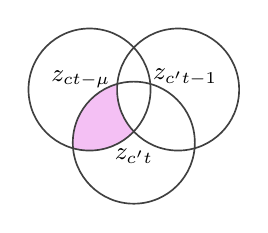
\begin{tikzpicture}[line cap=round,line join=round]
  %--- parámetros geométricos
  \def\R{1.55}
  \def\sep{2.25}
  \def\drop{1.35}

  % Etiquetas bajo los diagramas SUPERIORES
  \pgfmathsetmacro{\UNDERPAD}{0.35}
  \pgfmathsetmacro{\yunder}{\drop + \R + \UNDERPAD}

  % Controles de la zona TE (parte inferior)
  \def\yTE{-5.6}
  \pgfmathsetmacro{\TEeqoffsetBelow}{0.9}

  \tikzset{
    outline/.style={draw=black!75,line width=0.6pt},
    lab/.style={font=\Large, text=black!85}
  }

  % posiciones fila superior
  \def\xA{-8} \def\xB{-2} \def\xC{4} \def\xD{10}

  % ---- Conjunto inferior (TE)
  \pgfmathsetmacro{\xCenter}{(\xA+\xD)/2}
  \begin{scope}[scale=0.5]
    \coordinate (L) at (-\sep/2,0);
    \coordinate (R) at ( \sep/2,0);
    \coordinate (B) at (0,-\drop);
    \begin{scope}[blend group=screen]
      \begin{scope}
        \clip (B) circle (\R);
        \clip (L) circle (\R);
        \fill[softred, fill opacity=0.90, even odd rule] (-6,-7) rectangle (6,4) (R) circle (\R);
        \fill[softblue, fill opacity=0.90, even odd rule] (-6,-7) rectangle (6,4) (R) circle (\R);
      \end{scope}
    \end{scope}
    \draw[outline] (L) circle (\R);
    \draw[outline] (R) circle (\R);
    \draw[outline] (B) circle (\R);
    % Etiquetas internas (TE)
    \node[font=\small, align=center] at ([xshift=-0.22cm,yshift= 0.26cm] L) {$\ve{z}_{ct-\mu}$};
    \node[font=\small, align=center] at ([xshift=0.18cm, yshift=0.30cm] R) {$\ve{z}_{c't-1}$};
    \node[font=\small, align=center] at ([yshift=-0.34cm] B) {$z_{c't}$};
  \end{scope}


\end{tikzpicture}